\section{}
% Consider the PID and I-PD controllers shown below, each connected to a standard
% first-order system plant Gp(s) = 1/(τs + 1):

% Taking the parameter values as τ = 0.1, kp = 0.5, ki = 1, kd = 0.1, set up a Simulink diagram
% for each design, using a Step block for the reference r input, and two Scope blocks to record
% u and y. Include a sketch or screenshot of both designs.
% (b) Now run both simulations for the reference step input r(t) = 1+(t), and provide plots for y
% and u for each case. How does the performance of the two designs compare?

Consider the PID and I-PD controllers shown below, each connected to a standard
first-order system plant $G_p(s) = \frac{1}{\tau s + 1}$:
\begin{figure}[h]
    \centering
    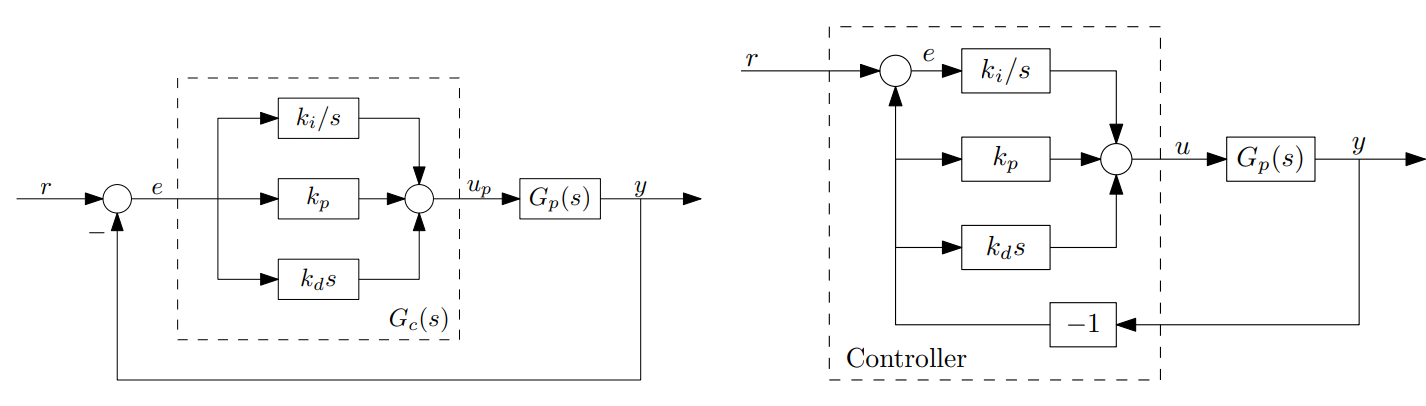
\includegraphics[width=0.8\linewidth]{Questions/Figures/Q1ProblemDiagram.png}
\end{figure}
\begin{enumerate}[label=(\alph*)]
    \item Taking the parameter values as $\tau = 0.1, k_p = 0.5, k_i = 1, k_d = 0.1$, set up a Simulink diagram
    for each design, using a Step block for the reference $r$ input, and two Scope blocks to record
    $u$ and $y$. Include a sketch or screenshot of both designs.
    \item Now run both simulations for the reference step input $r(t) = 1+(t)$, and provide plots for $y$
    and $u$ for each case. How does the performance of the two designs compare?
\end{enumerate}

\subsection{}
The Simulink diagram for the PID controller is shown in Figure \ref{fig:Q1PIDDiagram}.
\begin{figure}[h]
    \centering
    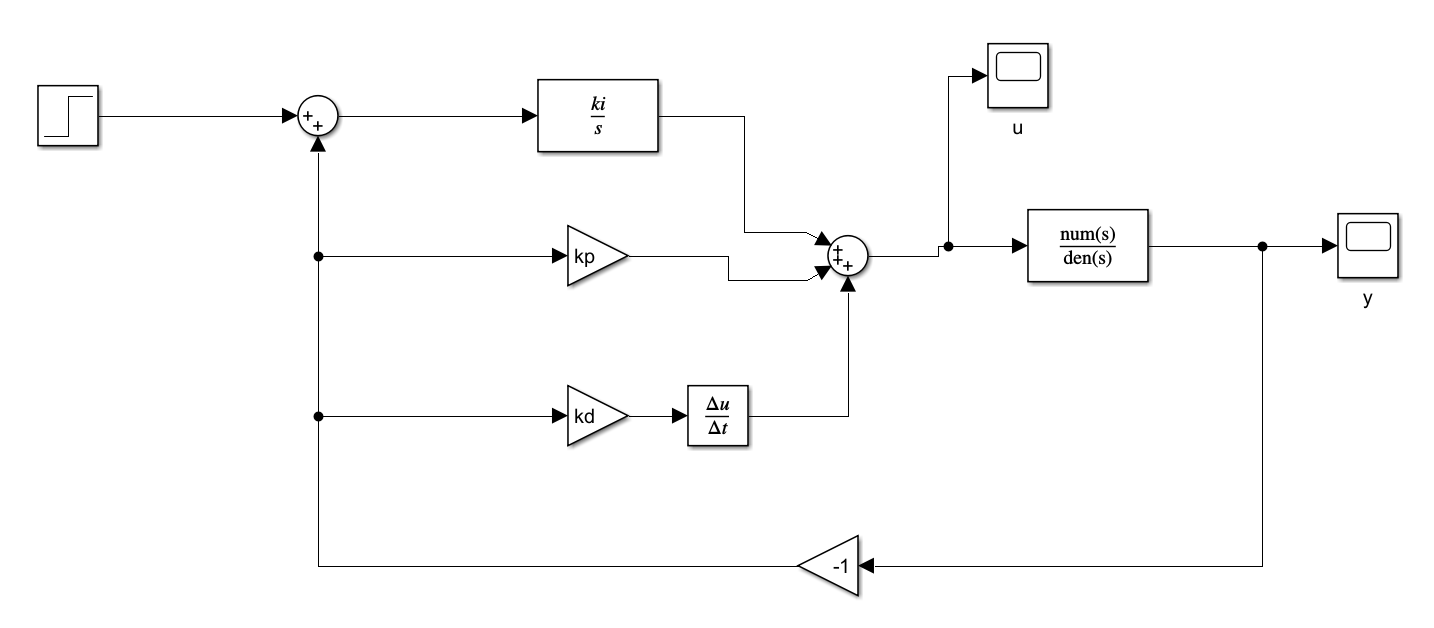
\includegraphics[width=0.8\linewidth]{Questions/Figures/Q1IPDDiagram.png}
    \caption{Simulink diagram for the PID controller}
    \label{fig:Q1PIDDiagram}
\end{figure}
The Simulink diagram for the I-PD controller is shown in Figure \ref{fig:Q1IPDDiagram}.
\begin{figure}[h]
    \centering
    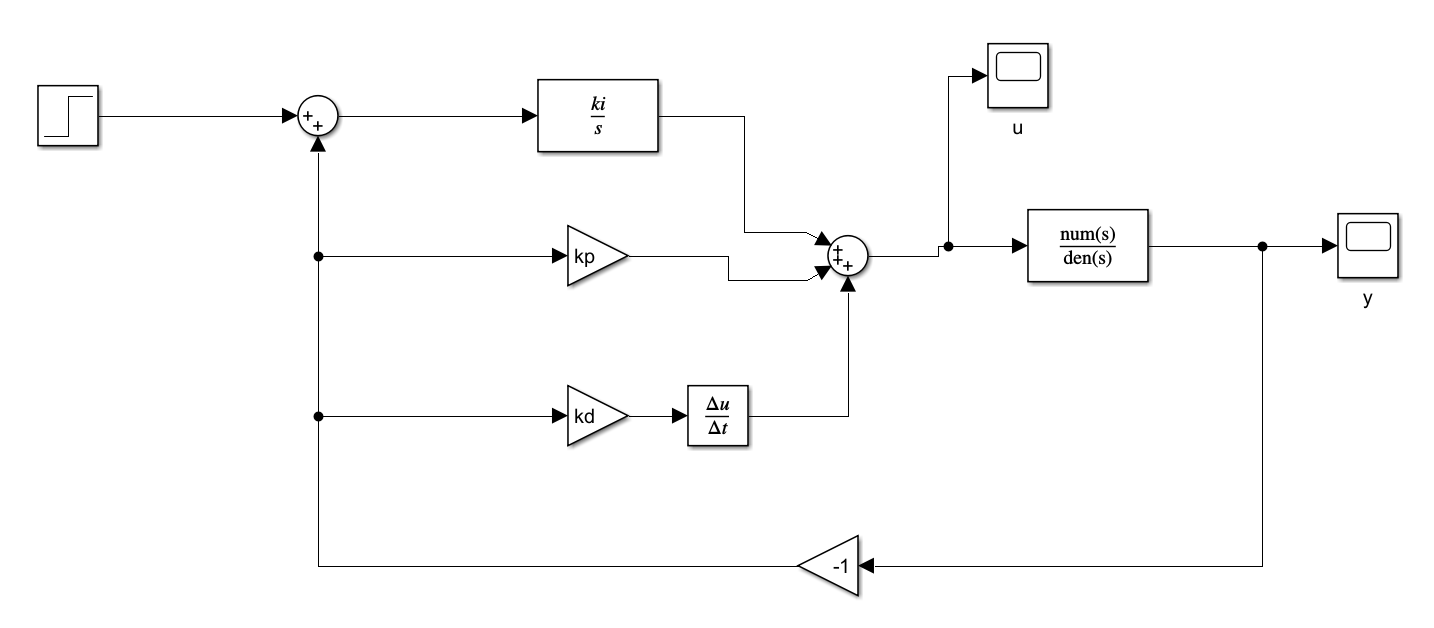
\includegraphics[width=0.8\linewidth]{Questions/Figures/Q1IPDDiagram.png}
    \caption{Simulink diagram for the I-PD controller}
    \label{fig:Q1IPDDiagram}
\end{figure}

\subsection{}
The scopes for the PID controller are shown in Figure \ref{fig:Q1PIDScopes}.
\begin{figure}[h]
    \centering
    \begin{subfigure}[b]{0.45\linewidth}
        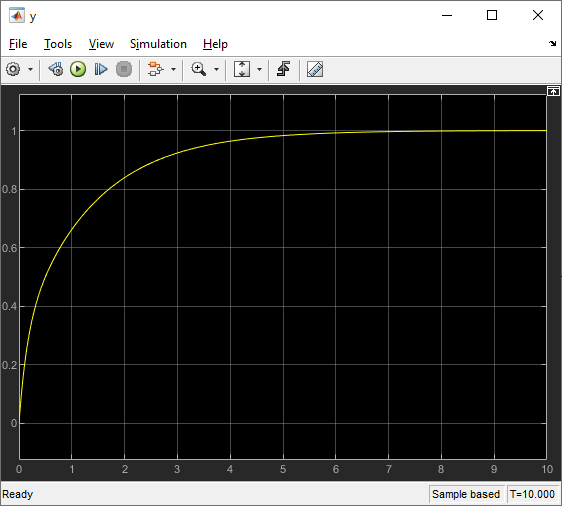
\includegraphics[width=\linewidth]{Questions/Figures/Q1PIDy.png}
        \caption{Response of $y$ to a step input $r(t) = 1_{+}(t-1)$}
    \end{subfigure}
    \begin{subfigure}[b]{0.45\linewidth}
        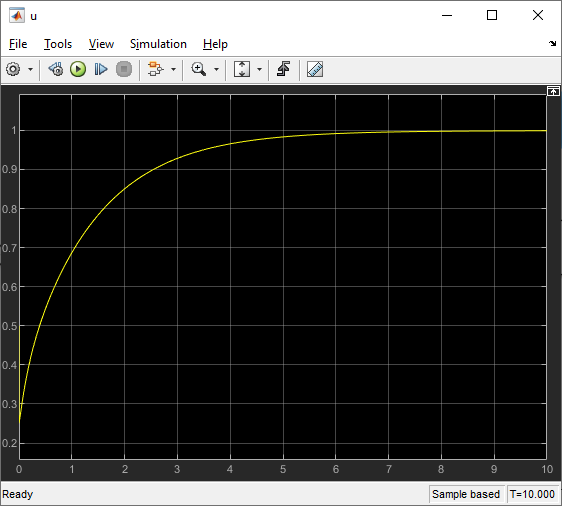
\includegraphics[width=\linewidth]{Questions/Figures/Q1PIDu.png}
        \caption{Response of $u$ to a step input $r(t) = 1_{+}(t-1)$}
    \end{subfigure}
    \caption{Scopes for the PID controller}
    \label{fig:Q1PIDScopes}
\end{figure}

The scopes for the I-PD controller are shown in Figure \ref{fig:Q1IPDScopes}.
\begin{figure}[h]
    \centering
    \begin{subfigure}[b]{0.45\linewidth}
        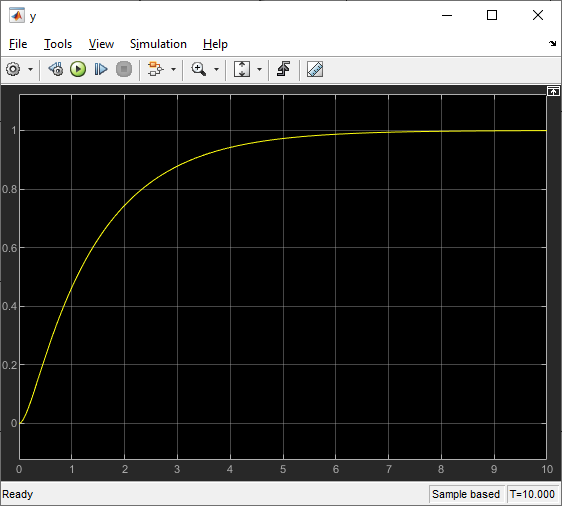
\includegraphics[width=\linewidth]{Questions/Figures/Q1IPDy.png}
        \caption{Response of $y$ to a step input $r(t) = 1_{+}(t)$}
    \end{subfigure}
    \begin{subfigure}[b]{0.45\linewidth}
        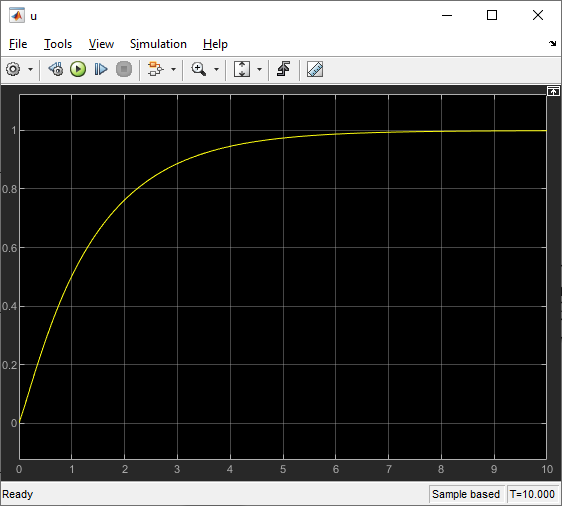
\includegraphics[width=\linewidth]{Questions/Figures/Q1IPDu.png}
        \caption{Response of $u$ to a step input $r(t) = 1_{+}(t)$}
    \end{subfigure}
    \caption{Scopes for the I-PD controller}
    \label{fig:Q1IPDScopes}
\end{figure}

The I-PD controller is smoother than the PID controller. If a step response of 
$r= 1_{+}(t-1)$ is used the PID has a large spike as shown in Figure \ref{fig:Q1BadScopes}.

\begin{figure}[h]
    \centering
    \begin{subfigure}[b]{0.45\linewidth}
        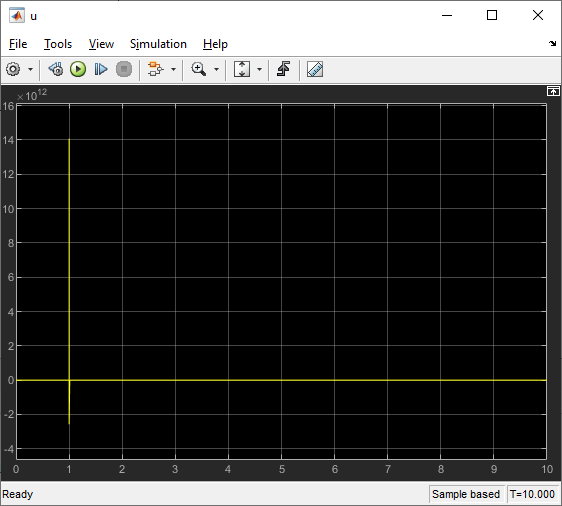
\includegraphics[width=\linewidth]{Questions/Figures/Q1PIDuBad.png}
        \caption{Response of $u$ to a step input $r(t) = 1_{+}(t-1)$}
    \end{subfigure}
    \begin{subfigure}[b]{0.45\linewidth}
        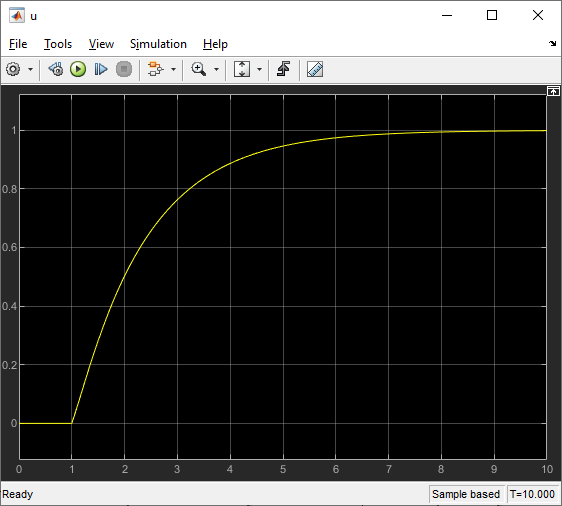
\includegraphics[width=\linewidth]{Questions/Figures/Q1IPDuBad.png}
        \caption{Response of $u$ to a step input $r(t) = 1_{+}(t-1)$}
    \end{subfigure}
    \caption{Scopes for the PID and I-PD controller with a step input $r(t) = 1_{+}(t-1)$}
    \label{fig:Q1BadScopes}
\end{figure}    